\cotefile{10}
\scanpage{171}
% archive sheet number: 170
topologique de $U$) dans $k$ (et $=$ sur $k$). Ainsi
on a un \deleted{\unsure{application}} homomorphisme d'algèbres
commutatives de $A$ dans l'algèbre des fonctions
\deleted{de} $G$ à valeurs dans $k$, transformant $1$ en $1$, compatible
d'ailleurs avec l'application diagonale et
l'augmentation, enfin aussi avec $\unsure{\nu|v|\vee}$. Dire que
c'est injectif signifie précisément que
$G$ est total dans $\underline U$. Noter que $G$ est exactement
l'ensemble de \uline{tous} les caractères de $A$
(qui est un groupe grâce à l'application
diagonale dans $A$ !) avec la topologie ``faible''
dire donc que $A\to\text{fonctions sur }G$ est
biunivoque signifie aussi que la transformation
de Gelfand \deleted{de} $A$ est biunivoque (si p. ex. $A$
est à \uline{engendrement fini sur $k$}, \deleted{\unsure{celà signifie que}}
\inserted{$k$ algébriquement}
% slanted
\margin{interpréter ceci en termes \unsure{d'associabilité|d'associativité} tensorielle $ {\unsure{K|k}}^{\underline U}$}
\uline{clos}, ceci signifie simplement que $A$ n'a pas
d'éléments nilpotents non nuls (si $x,\deleted{\unsure{\in|x'}}\in V$, $x'\in V'$
sont tels que $x'$ n'est pas orth. au plus
petit sous-\unsure{truc} de $V$ contenant $x$,
alors la $=$ ci-dessus est vraie pour
\[
x\otimes x\in V\otimes V\quad\text{et}\quad x'\otimes x'\in V'\otimes V'\,;
\]
contre-exemple \inserted{en car. $p\ne0$} à partir de $\underline A=k[X]/X^p\deleted{\unsure{-I}}$
\deleted{\unsure{$I$ puissance $p$ de l'idéal maximal|$I$ puissance pme de l'idéal maximal} $I=(X)^p$}
\deleted{$I$ l'idéal \unsure{maximal},} avec l'hom. diagonal naturel $\unsure{\leadsto}$ ; y-a-t-il un
\margin{???} contre-exemple en car. $0$ ?)

\scanpage{172}
% archive sheet number: 171
\deleted{\unsure{En te}} Si $\underline G$ est total dans $\underline U$, \inserted{i.e. $A$ est une algèbre de fonctions sur $G$,} alors la classe $\underline K^{U}$ s'identifie,
avec \deleted{toutes} ses structures, à la classe des \deleted{\unsure{rep}}
$G$-modules \inserted{de dim finie} tels que les \unsure{coéfficients|coëfficients|coefficients} \deleted{\unsure{en sont|sont}}
\deleted{\unsure{membres}} soient $\in A$.

Ainsi, une $\underline K$-hyperalgèbre $\underline U$ définit
un \uline{groupe} $G$, et une algèbre \inserted{\unsure{avec $1$|avec $1$,}} $A_0(G)$ de fonctions
sur $G$ à valeurs dans $k$, séparant les $\mathrm{p}^{\mathrm{ts}}$ de $G$,
\margin{\deleted{\unsure{à vérifier}}}
telle que \unsure{tt|ts} caractère \deleted{\unsure{que tt caractère de $A_0$ soit}} de $A_0$ soit défini
\deleted{stable sous $\nu$, et \unsure{ses translatées à g. et à droite}}
\inserted{par un $\mathrm{p}^{\mathrm{t}}$ de $G$, $A_0$ stable par $\unsure{\nu|v|\vee}$, et telle que}
% slanted
\margin{ceci \uline{implique} que $A_0$ est stable sous translations g. et dr.}
telle que $f\in A_0$ implique $f(xy)\in A_0\otimes A_0$. Alors
tout $\underline U$-module permis \uline{définit} un $\underline G$
module, permis pour $A_0$, [et la réciproque
est vraie si $G$ est \deleted{dense} \inserted{total} dans $U$].

\uline{Renversons la vapeur} partons d'un groupe
$G$ avec une algèbre $A_0$ ayant les propriétés
précédentes. Considérons la catégorie des
$G$-modules permis. Il lui correspond
une $\underline K$-algèbre $\underline U$, et
\diagram{\begin{tikzcd}[ampersand replacement=\&,row sep=small]
G \arrow[r] \& \underline U.\\
A_0 \& \underline A \arrow[l]
\end{tikzcd}}

Je dis que $G\to\underline U$ est une bijection
de $G$ sur \deleted{\unsure{un}} $G(\underline U)$ (éléments inversibles
de $U$ tels que $\delta(s)=s\otimes s$). Que ce
soit injectif résulte du fait que $A_0$
sépare les $\mathrm p^{\mathrm{ts}}$ de $G$, il est trivial que $G$
est appliqué dans $G(\underline U)$, \deleted{\unsure{p|pour}} montrons que
c'est surjectif. Comme tt caractère de $A_0$
provient de $G$, il suffit de prouver que $A\to A_0$

\scanpage{173}
% archive sheet number: 172
est bijectif. Ceci résulte de qqe chose de
plus général, voir plus bas.

Ainsi, on a identification des \uline{groupes} $G$
avec une algèbre $A_0$ de fonctions de $G$ dans $k$,
satisfaisant aux conditions précédentes, et
\uline{certains} \deleted{$\unsure{\underline U}$} $K$-anneaux $\underline U$

\uline{N.B.} Soit $\underline U$ un anneau \inserted{\unsure{linéairemt|linéairement}} \unsure{topologisé|topologique}
complet ayant un syst. fond. de
voisinages de $0$ \inserted{$\unsure{I}$} tels que les $U/I$ sont
de dim finie, $A$ la coalgèbre duale
(réunion \unsure{filtrante|filtrée} de ses sous-coalgèbres de
dim finie). Les $\underline U$-modules
permis sont les modules unitaires
sur $A$ de dim. finie sur $k$.

Soit $\Omega$ une \deleted{\unsure{bialgèbre}} \inserted{\unsure{$k$-algèbre|algèbre}} associative avec
$1$, considérons la classe des $\Omega$-modules
unitaires \deleted{Soit} de dim finie sur $k$.
Soit $A$ l'ensemble des formes sur $\Omega$
coefficients de représentations linéaires
de \uline{dim. finie} de $\Omega$. La multiplication
de $\Omega$ est continue pour $\sigma(\Omega\otimes\Omega,A\otimes A)$
et $\sigma(\Omega,A)$, i.e. on a un
hom naturel $A\unsure{-|\to} A\otimes A$, comme
on vérifie aussitôt (on est ramené
au cas de $\Omega=L_{k}(V)$, $V$ de dim
finie sur $k$).
\inserted{de plus \unsure{$A$ est} réunion \unsure{filtrante} de ses sous-coalgèbres de dim finie}
Alors, les $\Omega$-modules
unitaires \deleted{\unsure{de dim finie}} \deleted{\unsure{sont exactement les}} de

\scanpage{174}
% archive sheet number: 173
dim. finie sont exactement les coalgèbres \unsure{unitaires}
sur le comodule $A$ qui sont de dim finie
sur $k$. Donc c'est identique à la classe des
$\widehat\Omega$-modules permis, où $\widehat\Omega$ est le
complété de $\Omega$ pour $\sigma(\Omega,A)$.

\deleted{Considérons \unsure{la classe des comodules}}
\deleted{\unsure{unitaires sur une}}
Plus généralement, soit $\Omega$ une \unsure{$k$-algèbre}
avec $1$, \deleted{et soit $A_0$ une partie de $\Omega'$}
\deleted{\inserted{sous-espace de}} \deleted{\unsure{jouissant des propriétés}}
Les \unsure{coéfficients|coefficients} de représentations
\deleted{\unsure{sati}} de dim finie de $\Omega$ sont les
formes $f$ qui, par ``opération'' \deleted{\unsure{à}} gauche
\unsure{de} $\Omega$ ($\langle u,v*f\rangle=\langle uv,f\rangle$) engendrent un
sous-espace de dim finie \deleted{(s'il existe \unsure{un}}
% slanted
\margin{\[\begin{aligned}v*f_{x,x'}&=f_{vx,x'},\\ f_{x,x'}*v&=f_{x,{}^tv.x'}\end{aligned}\]}
(dans cet énoncé, on peut remplacer ``gauche''
par ``droite'' \inserted{ou ``bilatère''}), ou encore telles que
$f(uv)$ soit $\in\Omega'\otimes\Omega'$ (on a vu que
c'est nécessaire, car $f(uv)\in A\otimes A$ ;
c'est suffisant, car si $\deleted{\unsure{\angle}} f(uv)=
\sum f_i(u)g_i(v)$, alors
\[
\langle u,v*f\rangle=\sum_i\langle u,f_i\,g_i(v)\rangle,\quad\text{donc}
\]
$v*f=\sum c_i f_i$ varie dans un espace
de dim finie. --- Ceci dit,
soit $A_0$ un \deleted{\unsure{partie}} \inserted{sous-espace} de $\Omega'$ tel
que $f\in A_0$ implique $f(uv)\in A_0\otimes A_0$.
Alors $A_0$ est une sous-coalgèbre de $A$.$\unsure{\rho|\wp}$
% margin note written sideways
\margin{$\rho$ Alors $A_0\unsure{\to|\text{ est}}$ réunion \unsure{filtrante} de ses sous-coalgèbres de dim finie (car c'est vrai pour $A$, on prend les intersections avec $A_0$ !)}
% slanted
\margin{En passant, on obtient, si $A_0$ est un sous-espace de $A$, il revient au $=$ de dire que c'est une sous-co-algèbre, ou que c'est invariant par translations gauches et droites.}

\scanpage{175}
% archive sheet number: 174
\deleted{Supposons $A_0$ \unsure{fblt} dense dans $\Omega'$, i.e. $A_0$ en dualité avec $\Omega$}
Soit $K$ la classe des $\Omega$-modules $V$ \inserted{de dim. finie sur $k$} tels que
pour $x\in V$, $x'\in V'$, $f_{xx'}$ soit dans $A_0$. Cette
classe est isomorphe à la classe des $A_0$-comodules
(un tel module définit un
comodule sans hyp. sur la dimension ;
la réciproque marche, grâce à la dimension
finie). C'est donc aussi la classe des
$\widehat\Omega$-modules, où $\widehat\Omega$ est le complété
\deleted{\unsure{faible}} de $\Omega$ pour $\sigma(\Omega,A_0)$.

\unsure{On va interpréter|Or on interprète} autrement la donnée
d'un $A_0$ comme ci-dessus. $A_0$ définit, \inserted{on l'a vu,}
un ``groupe de représentations'' de dim finie
de $\Omega$ (i.e. classe de représentations stable
\unsure{par|sous} équivalence, passage aux sous-trucs et
quotients, sommes directes). Supposons
donné réciproquement un tel groupe $\unsure{\mathscr G|\mathcal G|G}$.
Soit $A_0$ l'ensemble des coefficients de
\unsure{ttes} les représentations de $\mathscr G$. \deleted{Alors} Je dis
que $A_0$ satisfait aux conditions précédentes :
en effet, \inserted{\textsuperscript{\unsure{(2)|(1)}}} si $f$ est un coéfficient d'une
représentation de dim finie de $\Omega$ sur $V$,
on a vu que \deleted{$\delta f=\sum f_i\otimes f'_i$, les}
\deleted{$f_i$ et $f'_i$ coefficients de la \unsure{même} représentation.}
\inserted{\unsure{les sommes de coefficients|les sommes de coéfficients} de la}
représentation forment déjà une coalgèbre

\scanpage{176}
% archive sheet number: 175
\deleted{de plus}, \textsuperscript{(1)} une somme de \deleted{tels} coefficients de
représentations, dans $V$, resp $W$ est un
coefficient d'une représentation dans $V\oplus W$. ---

\deleted{De plus, les}
Si on était \uline{parti} de $A_0$, puis passé à $\unsure{\mathscr G|\mathcal G|G}$,
on \unsure{retrouve son|retombe sur} $A_0$. Prouvons que partant de
$\mathscr G$, construisant $A_0$, alors \deleted{toute} représentation
de dim finie de $\Omega$ dont les coefficients
sont dans $A_0$, est dans $\mathscr G$. \deleted{\unsure{Démonstration|Dire}}
\deleted{par récurrence sur la dimension de $V$ :}
\deleted{Si $\dim V=1$, alors}

\uline{Lemme} 1 Toute représentation $\in\mathscr G(A_0)$ est
contenue dans une somme directe finie
représentations contenues dans $A_0$ (où
$\Omega$ opère par \unsure{cogénération|coopération|opération}) (On prend
une base $(e'_i)$ de $V'$, et on
prend la somme des représentations $x\unsure{-|\mapsto|\to} f_{x,e'_i}$)

Pour prouver $\deleted{\unsure{\mathscr G\subset}}\mathscr G(A_0)\subset\mathscr G$ on est ramené
au cas d'une représentation \uline{contenue}
dans $A_0$, à prouver qu'elle est $\in\mathscr G$.
Pour ceci, on note que \uline{lemme 2} toute
représentation \inserted{de dim finie} contenue dans $A_0$ est quotient
d'une somme \inserted{finie} de repr. \uline{monogènes}
contenues dans $A_0$ (trivial).

On est donc ramené au cas d'une
représentation dans $\Omega*f$, où $f\in A_0$.
On a $f=f_{xx'}$, $x,x'\in V$, $V$ \unsure{espace} \deleted{\unsure{de|d'une}}

\scanpage{177}
% archive sheet number: 176
d'une représentation \deleted{dans} appartenant à $\unsure{\mathscr G|\mathcal G}$. \unsure{Alors|Mais},
en vertu de $u*f_{x,x'}=f_{ux,x'}$, \deleted{\unsure{la}}
la représentation de $\Omega$ dans $\Omega*f$ est quotient
de la représentation donnée dans $V$, donc est
dans $\mathscr G$. CQFD.

\figure{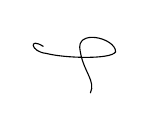
\begin{tikzpicture}[x=1cm,y=1cm]
\draw[line cap=round] (0.10,0.19) .. controls (-0.09,0.31) and (-0.06,0.12) .. (0.14,0.10) .. controls (0.37,0.04) and (0.96,0.02) .. (1.02,0.12) .. controls (1.02,0.30) and (0.50,0.42) .. (0.57,0.13) .. controls (0.61,-0.13) and (0.77,-0.25) .. (0.70,-0.40);
\end{tikzpicture}}

Repassons au groupe $G$. \deleted{\unsure{muni d'une}} Il
revient au \deleted{$=$ \unsure{de se donner}} \inserted{\unsure{pour|même}} un sous-espace $A_0$
du \deleted{$\unsure{G^k}$} dual $G^k$ de $G^{(k)}=k(G)$, de
dire que c'est l'ensemble des coefficients
d'un ``groupe de représentations'' \inserted{$\underline{\mathscr G}$} de $G$
(au sens ci-dessus), ou que les
fonctions $f(uv)$ \inserted{sur $G\times G$,} pour $f\in A_0$, sont dans
$A_0\otimes A_0$, et la donnée d'un tel $A_0$
est équivalente à \deleted{\unsure{un tel}} d'un $\underline{\mathscr G}$.
\deleted{\unsure{Si on veut que}} Dire que $\underline{\mathscr G}$ est
\uline{stable par produits tensoriels}, signifie
que $A_0$ est \uline{stable sous multiplication},
i.e. est une algèbre, \unsure{commtve|commutve|commutative} ; dire que
$\underline{\mathscr G}$ est stable par \uline{passage à la contragrédiente}
signifie que \uline{$A_0$ est stable sous $\unsure{\nu|v|\vee}$} ;

\scanpage{178}
% archive sheet number: 177
dire que $\underline{\unsure{\mathscr G|\mathcal G}}$ contient la représentation triviale dans $k$,
signifie que $1\in A_0$. \deleted{Dire que} Si \deleted{\unsure{donc}}
ces conditions sont \unsure{vérifiées|satisfaites}, \inserted{(on dit que $\underline{\mathscr G}$ est un \uline{\unsure{clan|classe} de représentations})} \deleted{\unsure{on a une}} on a une
$K$-catégorie, dont la \deleted{\unsure{coalg.}} \inserted{algèbre} des coéfficients est
$A_0$. Le \uline{groupe structural} est \inserted{donc} l'ensemble des
caractères de $A_0$, soit $G'$, et on a $G\unsure{-|\to}G'$.
\deleted{\unsure{Donc}} \inserted{Par définition} \uline{la dualité de Tannaka\unsure{.|,} vaut si et
seulement si $G\to G'(A_0)$ est bijectif},
i.e. \uline{$G$ est exactement le groupe des
caractères de $A_0$}, i.e. $A_0$ sépare les $\mathrm p^{\mathrm{ts}}$
de $G$, et tt caractère de $A_0$ provient de $G$.

A quelles condition la structure sur $G$ définie
par la donnée de $\underline{\mathscr G}$, i.e. de $A_0$, est
elle une structure de \uline{groupe algébrique
linéaire}$\unsure{??|?}$
\deleted{\unsure{i.e. si applicable à la situation}}
\deleted{\unsure{définie par}} \inserted{Il faut, et il suffit que}
$A_0$ \uline{soit à engendrement fini} sur $k$.

% slanted
\margin{de nouveau, il est inutile de se restreindre au cas d'un $A_0$ défini sur $G$, un groupe, mais on \unsure{peut} partir d'un $A_0$ quelconque.}
On sait que il revient au $=$ que
\uline{$R$ soit à ``engendrement fini''} en tant
qu'ensemble de représentations, i.e. qu'il
existe une $V\in R$ telle que \deleted{tout}
$W\in R$ soit contenue dans un $\overset{\unsure{n}}{\otimes}V$ ;
Nécessaire, car si les $f_i\in A_0$ sont des
générateurs de $A_0$, et les $V_i$ des $\in R$

\scanpage{179}
% archive sheet number: 178
tels que \deleted{\unsure{le}} $f_i$ soit un coéfficient pour $V_i$, alors
il suffit de prendre $V=\sum V_i$. \deleted{\unsure{Nécessaire, car}} \inserted{Suffisant,}
car considérant \deleted{tous les coéfficients de la} \inserted{une base $(e_i)$} de $V$,
et les coéfficients $f_{e_i,e'_j}$, on voit que
tout coéfficient relatif à $\overset{\unsure{n}}{\otimes}V$ (donc à
un sous-truc ou un truc quotient) est
contenu dans l'algèbre engendrée par les
$f_{e_i,e'_i}$.
% slanted
\margin{par définition ou \unsure{paraphrase} de la multiplication dans la coalgèbre $A_0$, on a, pour \unsure{des} $A$-comodules $V,W$ et $x\,x'\,y\,y'$ dans $V\,V'\,W\,W'$,\[\begin{aligned}f_{x,x'}f_{y,y'}&=f_{x\otimes y,x'\otimes y'}.\ \text{\unsure{V.}}\\ f_{x,x'}\unsure{*}f_{y,y'}&=f_{x\otimes x',y\otimes y'}\ \text{\unsure{''}}\end{aligned}\]}
% slanted
\margin{\deleted{\illegible{1}} \uline{Lemme} 1. L'algèbre engendrée par les coefficients de la repr. dans $V$ est l'ensemble des coefficients dans \deleted{\unsure{tous}} les représentations $\overset{n}{\otimes} V$. De plus, les représentations \unsure{contenues} dans un \unsure{quotient} d'un $\overset n\otimes V$ forment une \uline{classe} de représentations.}

\uline{N.B.} \deleted{Soit} Si $G$ est algébrique linéaire
il a une représentation linéaire fidèle \deleted{\unsure{pour}}
\deleted{\inserted{\unsure{d'image fermée}}}, $\searrow\ \oplus$ \deleted{\unsure{induisant la structure ci-dessus, la représentation dans $V$.}}
\inserted{qui est un \uline{isomorphisme} $\updownarrow$ \unsure{onto.} au sens de l'énoncé des conditions équivalentes \unsure{barrées}.}
i.e. $G$ est
un sous-groupe ``fermé'' de $\mathrm{Gl}(V)$, avec
la structure algébrique induite (i.e. $A_0$ est
l'algèbre des polynômes en les fonctions
``coordonnées'' $g_{ij}$ et $\det(g_{ij})^{-1}$) : il
suffit de prendre \deleted{un \unsure{système (f) fini}}
\deleted{de générateurs de $A_0$, et une} $V$
comme ci-dessus, i.e. telle que $A_0$ soit
l'alg. engendrée par les \deleted{\unsure{fonctions}} $g_{ij}\in A_0$.
% slanted
\margin{en fait, il faut dire que \deleted{\unsure{toutes}} représentations de $R$ sont \uline{\unsure{exactt|exactement}} les représentations ``régulières'' du groupe algébrique $G$ défini de la façon voulue}
Il faut seulement montrer a) que $\det(g_{ij})^{-1}\in A_{\unsure{0}}$
ce qui résulte du fait que $\det(g_{ij})$ ne
s'annule pas sur $G$ donc \deleted{\unsure{est un inv.}} \inserted{son inverse}
est \deleted{\unsure{rationnelle}} régulière sur $G$ ; b) que
$\overline G\subset\mathrm{Gl}(W)$ est fermé pour la top.
de Zariski de $\mathrm{Gl}(W)$ (et $=$ dans $L(W)$,
pour la top de Zariski de $L(\unsure{V|W})$). Mais

\scanpage{180}
% archive sheet number: 179
celà résulte encore du fait que les fonctions
régulières sur $L(W)$ s'appliquent \uline{sur} les fonctions
régulières sur $G$,

\diagram{\resizebox{\linewidth}{!}{\begin{tikzcd}[ampersand replacement=\&,column sep=0.3em,row sep=1.0em]
\text{$K$-catégorie} \& \Longleftrightarrow \&
K\text{-}\overset{\inserted{\text{hyperalgèbre}}}{\deleted{\text{algèbre}}}\,\underline U
\arrow[r,Leftrightarrow] \& \substack{\text{hyperalgèbre commu-}\\\text{tative }A,\ \text{réun.}\\\text{filtrante }\ldotp\ldotp\ldotp\ldotp}\\
\& \substack{\text{\uline{cas particuliers}}\\[3pt]\text{\uline{Groupe pseudo-algébrique}}\\
(\text{cas où }G(\underline U)\ \deleted{\text{est}}\ \inserted{\text{total}}\ \text{dans }\underline U,\\
\text{ou encore }\underline A\ \text{soit }\unsure{p|\rho}\text{-radical, i.e.}\\
\text{l'intersection des noyaux des caractères}\\\text{de }A\text{ est réduite à }0)}
\arrow[u,Rightarrow] \& \& \\
\& \substack{\text{Groupe algébrique}\\(\text{si }\deleted{\unsure{\text{des}|\text{de}}}\ \text{plus }A\text{ est une }k\text{-}\\\text{algèbre de type fini})} \arrow[u,Rightarrow] \& \&
\end{tikzcd}}}
\margin{Si $A$ est une $k$-algèbre de type fini, \inserted{sur $k$ alg. clos,} pour qu'il s'agisse d'un groupe algébrique, (il faut et) il suffit que $A$ n'ait pas d'\unsure{élémts|éléments} nilpotents $\ne0$ ($k$ alg\textsuperscript{t.} clos est-il nécessaire ?) Ceci est-il automatiquement vérifié en caractéristique $0$ ???}

\scanpage{181}
% archive sheet number: 180
Considérons à nouveau une classe abélienne \deleted{\unsure{de}}
$\unsure{\mathcal K|\mathscr K|\mathcal R}$ dont les trucs soient tous de longueur finie.
Soit $I$ l'ensemble des classes de trucs indécomposables dans $\mathcal K$, soit $Z(I)$ le groupe libre
engendré par $I$. C'est un groupe ordonné $\unsure{\Gamma|F}$, et
d'après Remak-Schmidt, $\Gamma^+$ (l'ens. des
éléments positifs) est canoniquement isomorphe à l'ensemble des classes de trucs
$\in\mathcal K$ modulo isomorphisme, la somme dans
$\Gamma^+$ correspondant à l'opération de somme
directe. Si $\mathcal K$ est une classe de \deleted{\unsure{modules}}, \inserted{\unsure{vectoriels|modules} sur $k$ de dim finie sur $k$ avec structures suppl.}
et si on suppose que $k$ soit muni d'une
structure \unsure{$\mathcal K$|de $K$} privilégiée, alors $I$ a un
élément distingué $e$ ; si dans $K$, on a
une involution $\vee$ (le dual d'un \unsure{vectoriel|variable|module}
muni d'une structure $K$ est muni
d'une structure \unsure{d$K$|$K$}) alors $I$ est muni
d'une involution $i\unsure{-|\to}\check i$, et la
compatibilité de l'opération $\nu$ avec la structure
privilégiée de $k$ s'exprime par $\check e=e$.
\inserted{$\unsure{V|\nu}$ et $e$ \unsure{définissent|déterminent} involution et $e$ dans $\Gamma$}
\unsure{Noter|Notons} que sur $I$, il y a une fonction
privilégiée $n(i)=\dim M_i$, qui se
prolonge par linéarité à $\Gamma=Z(I)$ ;

\scanpage{182}
% archive sheet number: 181
sur $ {\Gamma}^+$, c'est la fonction ``dimension d'un
module''. Dans le cas \uline{où} on a un $e$,
on a $n(e)=1$, et si on a un $\unsure{\nu|v|\vee}$, on a
$n(\check i)=n(i)$.

$\unsure{\mathcal K|\mathscr K|\mathcal R}$ est bien définie si, en plus de
$I$ et de la fonction $n(i)$, on se donne un
représentant $M_i$ de chaque $i$ avec comme
module sous-jacent $k^{n(i)}$, et pour $i,j$ donnés,
un sous-groupe $\operatorname{Hom}_{j,\deleted{\unsure{j|k}}i}(k^{n(i)},k^{n(j)})$,
de façon que $\operatorname{Hom}_{\unsure{kj|kj\,j}}\times\operatorname{Hom}_{\unsure{ji|ij}}$ soit appliqué
par composition dans $\operatorname{Hom}_{ki}$, etc\ldots.

Supposons que dans $K$ on ait une
notion de produit tensoriel, alors
$\Gamma(K)$ est muni d'une loi d'anneau \inserted{associatif}
et commutatif, qui sur $\Gamma^+(K)$ \deleted{\unsure{p|y}} correspond
à la loi de produit tensoriel. $\underline n$ est une
fonction multiplicative sur $\Gamma^+$, et la
compatibilité avec $e$ \deleted{signifie} \inserted{implique} que $e$ est
une unité pour \deleted{\unsure{l'op}} la loi d'algèbre. La
compatibilité avec $\nu$ \deleted{signifie} \inserted{implique} que $\nu$ est
un automorphisme de l'algèbre $\Gamma$. Enfin
la compatibilité simultanée de
$e,\nu,\otimes$ implique que $i*\check i$ a toujours
\deleted{\unsure{p|pour}}pour composante non nulle suivant $e$.
$I$ est alors un ``\uline{hypergroupe discret}''

\scanpage{183}
% archive sheet number: 182
Si tout $M\in C$ est complètement réductible,
\inserted{et $C$ défini par un \uline{groupe} $\underline G$ avec une algèbre $A$ sur $G$,}
alors $\Gamma$ s'identifie à l'algèbre des \deleted{\unsure{coéfficients}}
\inserted{\unsure{combinaisons}} \deleted{caractères} linéaires des caractères (fonctions sur
$G$) des représentations \unsure{données|linéaires|degrés|dimensions} de $G$,
$\Gamma^+$ à \deleted{\unsure{un}} \inserted{l'ensemble des} caractères des représentations linéaires
de $G$ (avec conservation de \deleted{\unsure{toutes}} les
structures : $n(f)$ devient $f(e)$ ($e\in G$),
$\vee$ devient $\nu$, $e$ devient la fonction $1$ sur $G$,
\unsure{produits produit|produits produits} ; noter d'ailleurs qu'il
s'agit de fonctions centrales). Si p. ex
$G$ est un groupe algébrique semi-simple complexe,
on obtient une connaissance structurale
concrète de $\Gamma$, qui est l'algèbre des
fonctions régulières sur $T/W$, $T$ un
``tore'' maximal, $W$ le groupe de Weyl
(il faudrait essayer de trouver une
caractérisation intrinsèque simple des
caractères irréductibles, i.e. des $\in I$ ; pour
ceci, il faut mettre sur $T/W$ une
\margin{?} structure de hypergroupe, dont on
doit construire les caractères irréductibles)

Cas de $G=k^*$ ($k$ alg\textsuperscript{t} clos pour
simplifier). Alors $\Gamma(G)\simeq\text{algèbre du groupe }Z$
($I(G)\simeq Z$, avec \unsure{ttes} les structures).

\scanpage{184}
% archive sheet number: 183
% slanted
\margin{Caractéristique $0$ ?}
Cas de $G=k$ \inserted{($k$ alg\textsuperscript{t} clos pour simplifier)}. Une représentation rationnelle
de $k$ est unipotente, leur classification est donc
identique à celle des opérateurs unipotents,
ou encore des opérateurs nilpotents, i.e.
des modules sur $k[x]$ qui sont
annulés par une puissance convenable de $x$.
Donc les diviseurs élémentaires sont du type
$x^k$, donc $I\simeq {\unsure{N|\mathbb N}}^+$ (un représentant de $i$
\unsure{entier} $\in N^+$ étant $k[x]/{\unsure{x|X}}^i$). L'élément
neutre est $1,\in N^+$, l'involution l'identité.
Quelle est la multiplication ?
